\begin{titlepage}
\phantom.

\bigskip

\begin{center}
{\sc\LARGE Žilinská Univerzita v Žiline}
\medskip

{\sc\Large Fakulta riadenia a informatiky}

\vfill\vfill\vfill\vfill

{\sc\LARGE Bakalárska práca}

\medskip

{\large Študijný odbor: {\bf Informatika}}
\end{center}


\vfill\vfill\vfill\vfill


\phantom.\hfill

\begin{center}
{\large\bf Oľga Chovancová}

\medskip

{\large\bf Vizualizácia dát získaných pomocou SCADA systémov s~využitím HTML 5 štandartov}

\medskip

Vedúci: {\bf Ing. Juraj Veverka}\\
Tútor	\textbf{Ing. Patrik Hrkút, PhD.}
\medskip
 
\hfill
Reg.č. 5/2014
\hfill
Máj 2015
\hfill\phantom.
\end{center}

\hspace{1.7cm}\phantom.

\vspace{2.9cm}

\phantom.
\end{titlepage}
%%%%%%%%%%%%%%%%%%%%%%%%%%%%%%%%%%%%%%%%%%%%%%%%%%%%%%%%%%%%%%%%%%%%%%%%%%%%%%%%%%%%%%%%%%%%%%%%%%%%%%%%%%%%%%%%%%%%%%%%%%%%%%%%%%%%%%%%%%%%%%%%%%%%%%%%%%%%%%%%%%%%%%%%%%%%%%%%%%%%%%%%%%%%%%%%%%%%%%%%%%%%%%%%%%%%%%%%%%%%%%%%%%%%%%%%%%%%%%%%%%%%%%%%%%%%%%%%%%

%%%%%%%%%%%%%%%%%%%%%%%%%%%%%%%%%%%%%%%%%%%%%%%%%%%%%%%%%%%%%%%%%%%%%%%

%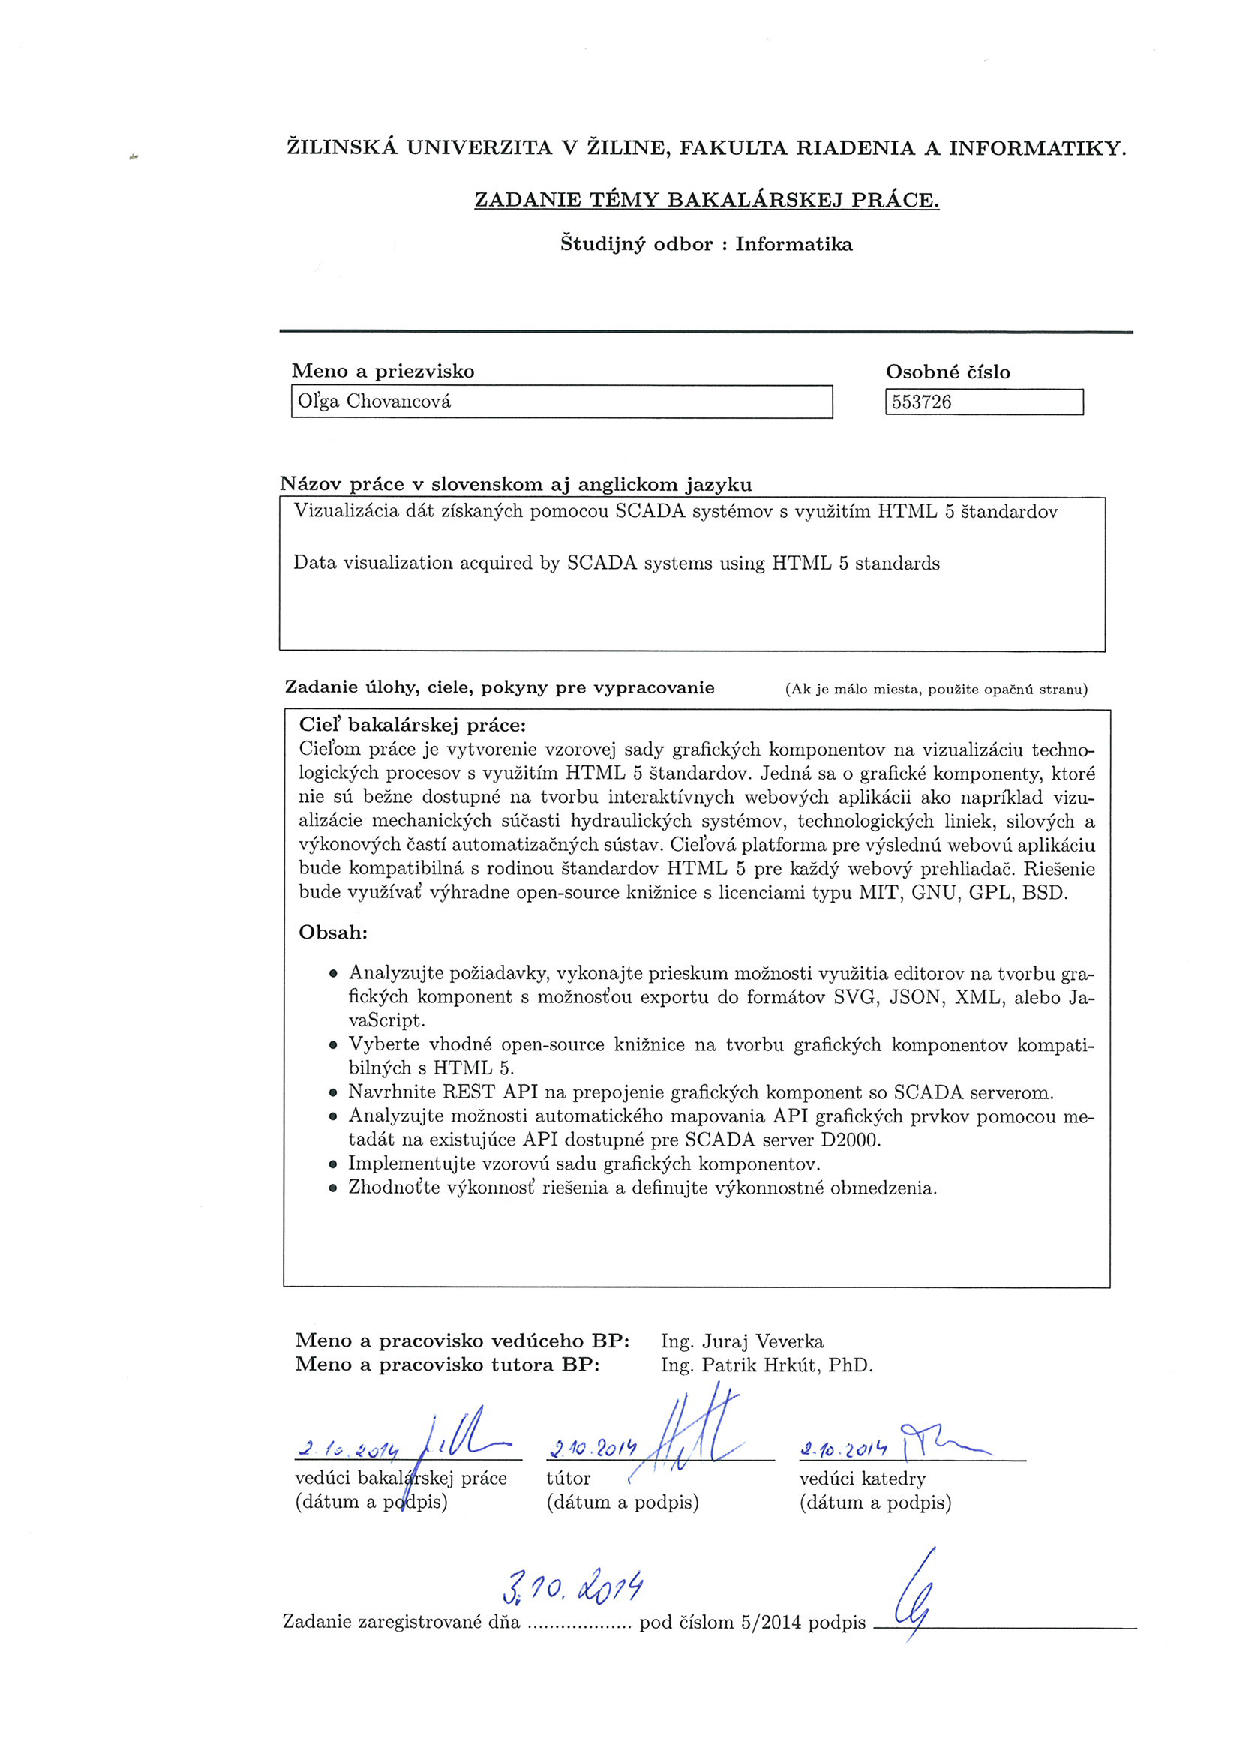
\includepdf{zadanie.pdf}

\newpage

\centerline{\bf Čestné prehlásenie}

\vspace{2em}

\noindent
Prehlasujem, že som bakalársku prácu \textit{Vizualizácia dát získaných zo SCADA systémov použitím HTML5 štandardov} vypracovala samostatne pod vedením Ing. Juraja Veverku, a uviedla v nej všetky použité literárne a iné odborné zdroje v súlade s právnymi predpismi, vnútornými predpismi Žilinskej univerzity a vnútornými aktmi riadenia Žilinskej univerzity a Fakulty riadenia a informatiky.

\vspace{2em}

\noindent
V~Žiline, dňa 15.05.2015
\hfill
Oľga Chovancová

\newpage


\newpage

\centerline{\bf Poďakovanie}
\vspace{2em}
\noindent
%Prehlasujem, že som túto prácu napísala samostatne a že som uviedola
%všetky použité pramene a literatúru, z~ktorých som čerpala. 

\bigskip

Na tomto mieste by som chcela poďakovať vedúcemu bakalárske práce Ing. Jurajovi Veverkovi za cenné pripomienky a odborné rady, ktorými prispel k vypracovaniu tejto bakalárskej práce. Taktiež ďakujem môjmu tútorovi Ing. Patrikovi Hrkútovi, PhD. Zároveň ďakujem mojej rodine a priateľom za ich nekonečnú podporu a trpezlivosť. 

\vspace{2em}

\noindent
V~Žiline, dňa 15.05.2015
\hfill
Oľga Chovancová